\documentclass[a4paper,11pt]{article}
\usepackage{graphicx}
\usepackage[backend=bibtex]{biblatex}
\usepackage{pgfplots}
\usepackage[strings]{underscore}
\usepackage[T1]{fontenc}
\usepackage{amsmath}

\addtolength{\oddsidemargin}{-.7in}
\addtolength{\evensidemargin}{-.7in}
\addtolength{\textwidth}{1in}

\addtolength{\topmargin}{-.7in}
\addtolength{\textheight}{1in}


\begin{document}

	
\title{Lambda Calculus Evaluator User Guide}
\date{\today}
\newpage

\maketitle
\Large{Code can be found at https://github.com/jonesy30/LambdaCalculator}
\section{Inputs}
To input a lambda symbol, type the \% symbol. This will automatically change to a $\lambda$.\\

Enter applications in the form \texttt{MN}, for example to input \texttt{3} applied to \texttt{x+1} input \texttt{(\% x.x+1)3}.\\

Enter multi-input abstractions in separate abstractions, so \texttt{$\lambda$xy.x*y} becomes \texttt{$\lambda$x.$\lambda$y.x*y}.\\

The following are a list of things you can use to build your term. Note: whitespace is ignored, variables are case sensitive (q is a different variable to Q).

\subsection{Value Options}
\begin{itemize}
	\item Boolean values: TRUE or FALSE (not case sensitive - true and TRUE are the same)
	\item Variables: Single-character values a-z and A-Z (capitals allowed)
	\item Numbers: Any positive number
\end{itemize} 

\subsection{Operations}
\begin{itemize}
	\item Arithmetic operations: + - / \^
	\subitem(note: 3x notation is not supported, should be input as 3*x)
	\item Parenthesis ( ) are supported
	\item Boolean operations: \& represents and, | represents or
	\item Comparison operations: > represents greater-than, < represents less-than, == represents equal to 
\end{itemize}

Note: arithmetic functions do not follow the expected order of operations (BODMAS or similar), so arithmetic calculations with more than one operation will likely not give you what you expect. This is a limitation with the code I didn't have time to fix - sorry!

\subsection{Types}
Types can be input alongside any variable in a lambda term in \texttt{x:type} form. The following types are supported (note: case should not matter):

\begin{itemize}
	\item int
	\item bool
	\item none
	\item $[type] -> [type]$ (for function type)
\end{itemize}

These types can be put alongside any variable in a lambda term, so an example lambda term with types is:
\begin{quotation} \texttt{($\lambda$x:int.x:bool)y:bool} \end{quotation}
(note: this term is invalid because of conflicting types, it is just given as an example).

\section{Interface Guide}

To use the interface, enter lambda terms in the \texttt{Enter expression here} box shown in Figure \ref{web_interface_no_input}, and click the \texttt{Check Expression} button (pressing enter on a keyboard should also work). The results will appear in the box underneath.\\

Different evaluation methods can be selected based on what you're wanting out of the interface. \texttt{Alpha Conversion Only} will not perform beta reduction, it will just return the alpha converted term. \texttt{Call by Value} and \texttt{Call by Name} are different methods of beta reduction, \texttt{Call by Name} works in the same way as Call by Need and Normal Order Reduction, and is selected by default. Call by Name will evaluate all terms to their normal form if one exists, this is not true for Call by Name.\\

\subsection{Results}

An example of the results given when a term is input is shown in Figure \ref{web_interface_input}. The result shows the evaluated term, valid typing states whether or not the term can be typed (meets typing rules defined in the lecture slides with no conflicting types across like-terms), and the type returned is the type of the \textbf{final term} output in the Results section. In order to find the typing context and beta evaluation steps, click either the \texttt{click here for evaluation details} or \texttt{click here} links next to the Result and Typing Context information (both of these links direct you to the same page).\\

Clicking either of these will open a new tab shown in Figure \ref{web_interface_more_information}, which gives details about the typing context and beta reduction steps which were used to reach the final result.

\subsubsection{Typing Context}

The typing context relates to the types which the program has found for each variable, throughout evaluation of \textbf{the whole evaluation}. This means that one variable could have multiple types, this is because the same variable refers to different objects in the expression, as explained in the interface.

\subsubsection{Beta Reduction Details}

This gives details about the steps carried out by the program to evaluate the term, starting with the type of beta reduction selected. This does not show evaluation of functions or the final arithmetic evaluation, instead focusing on the application of beta reduction rules.

\section{Error Messages}

Error messages can happen for a number of reasons, an example of which is shown in Figure \ref{web_interface_error}. The following is a list of all the possible error messages, what they mean, and what to do about them.

\begin{itemize}
	\item Mismatched brackets
	\subitem This is due to a syntax error and brackets not being matched properly - check to make sure you've closed all open brackets
	\item Syntax error
	\subitem This is an error from the underlying grammar parser, check to make sure your term is in the correct form and you aren't using multi-input abstractions, and that each abstraction is in the form $\lambda x.[term]$
	\item Normal form not found
	\subitem This occurs when the term cannot be evaluated because the normal form of the term does not exist. This could also occur due to extremely large lambda terms (over 20 nested abstractions)
	\item Invalid visitor selected
	\subitem This is a command line interface and shouldn't appear on the web interface, if it does try refreshing the page
	\item Something went wrong
	\subitem This is due to an exception other than those mentioned here. Congratulations, you've found a bug! Please don't blame me - I tried. Try re-entering the term, refreshing the page, or try a similar term
\end{itemize}

\begin{figure}[p]
	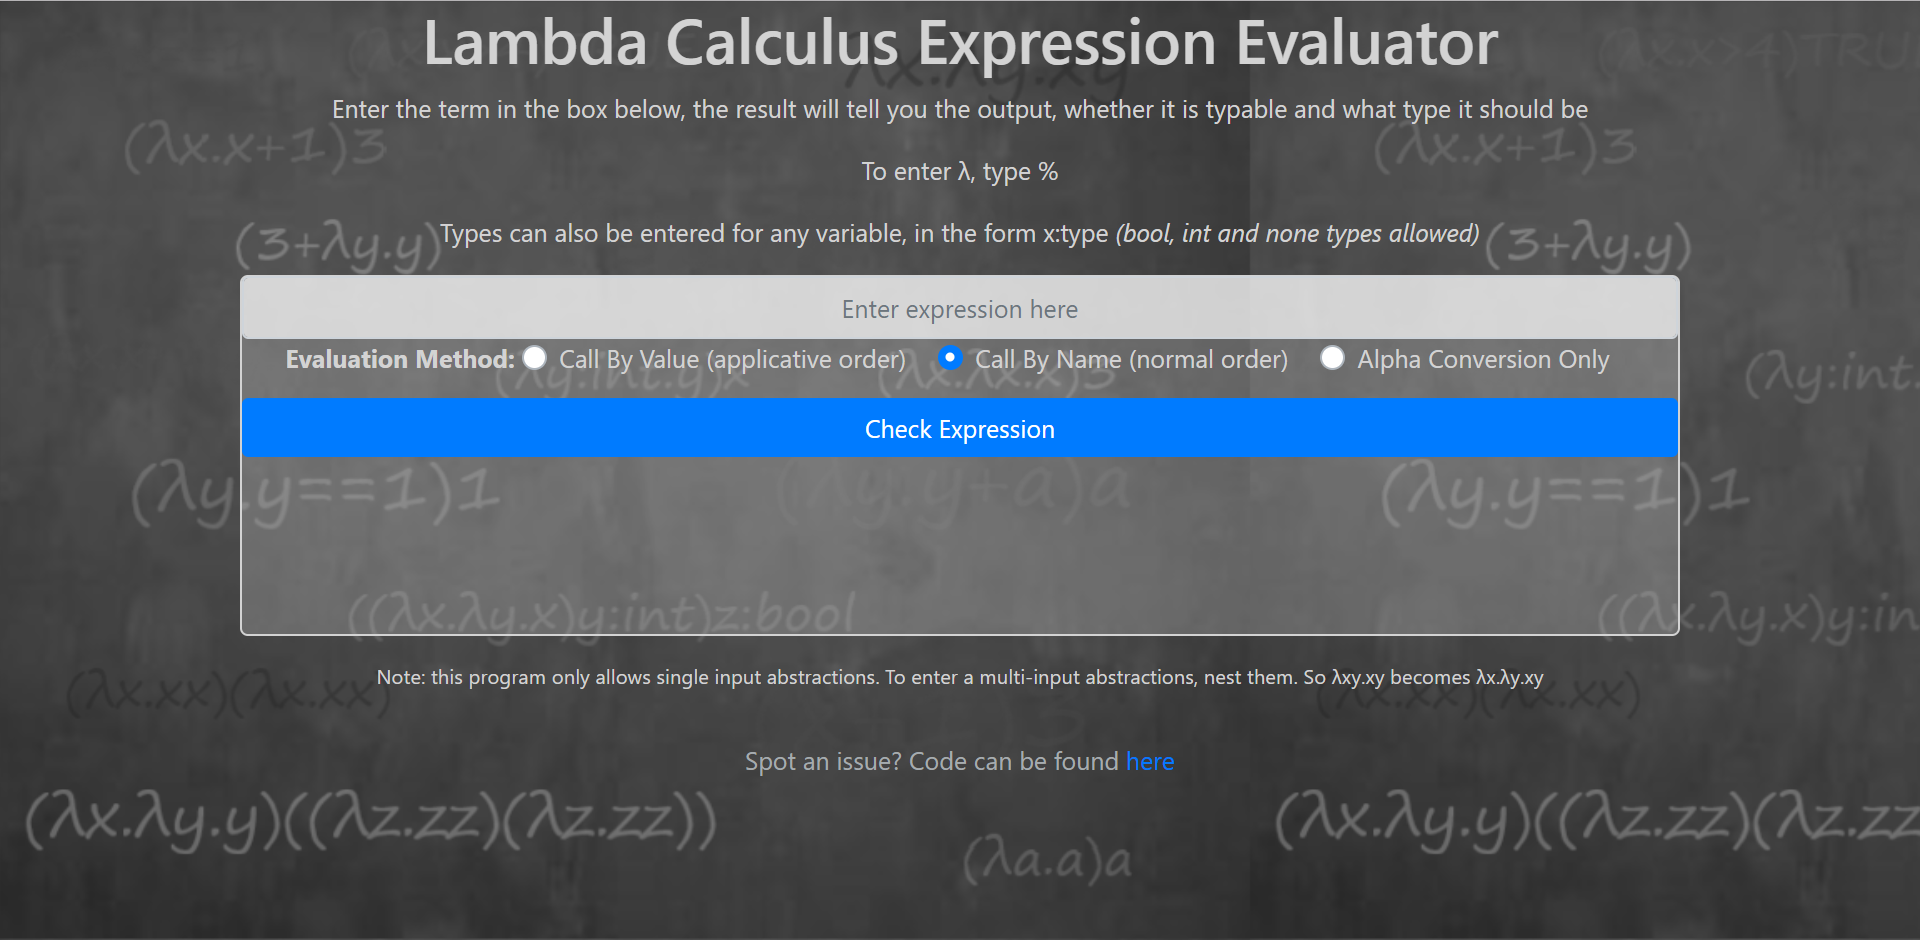
\includegraphics[scale=0.4]{images/web_interface_no_input}
	\centering
	\caption{Web Interface}
	\label{web_interface_no_input}
\end{figure}

\begin{figure}[p]
	\centering
	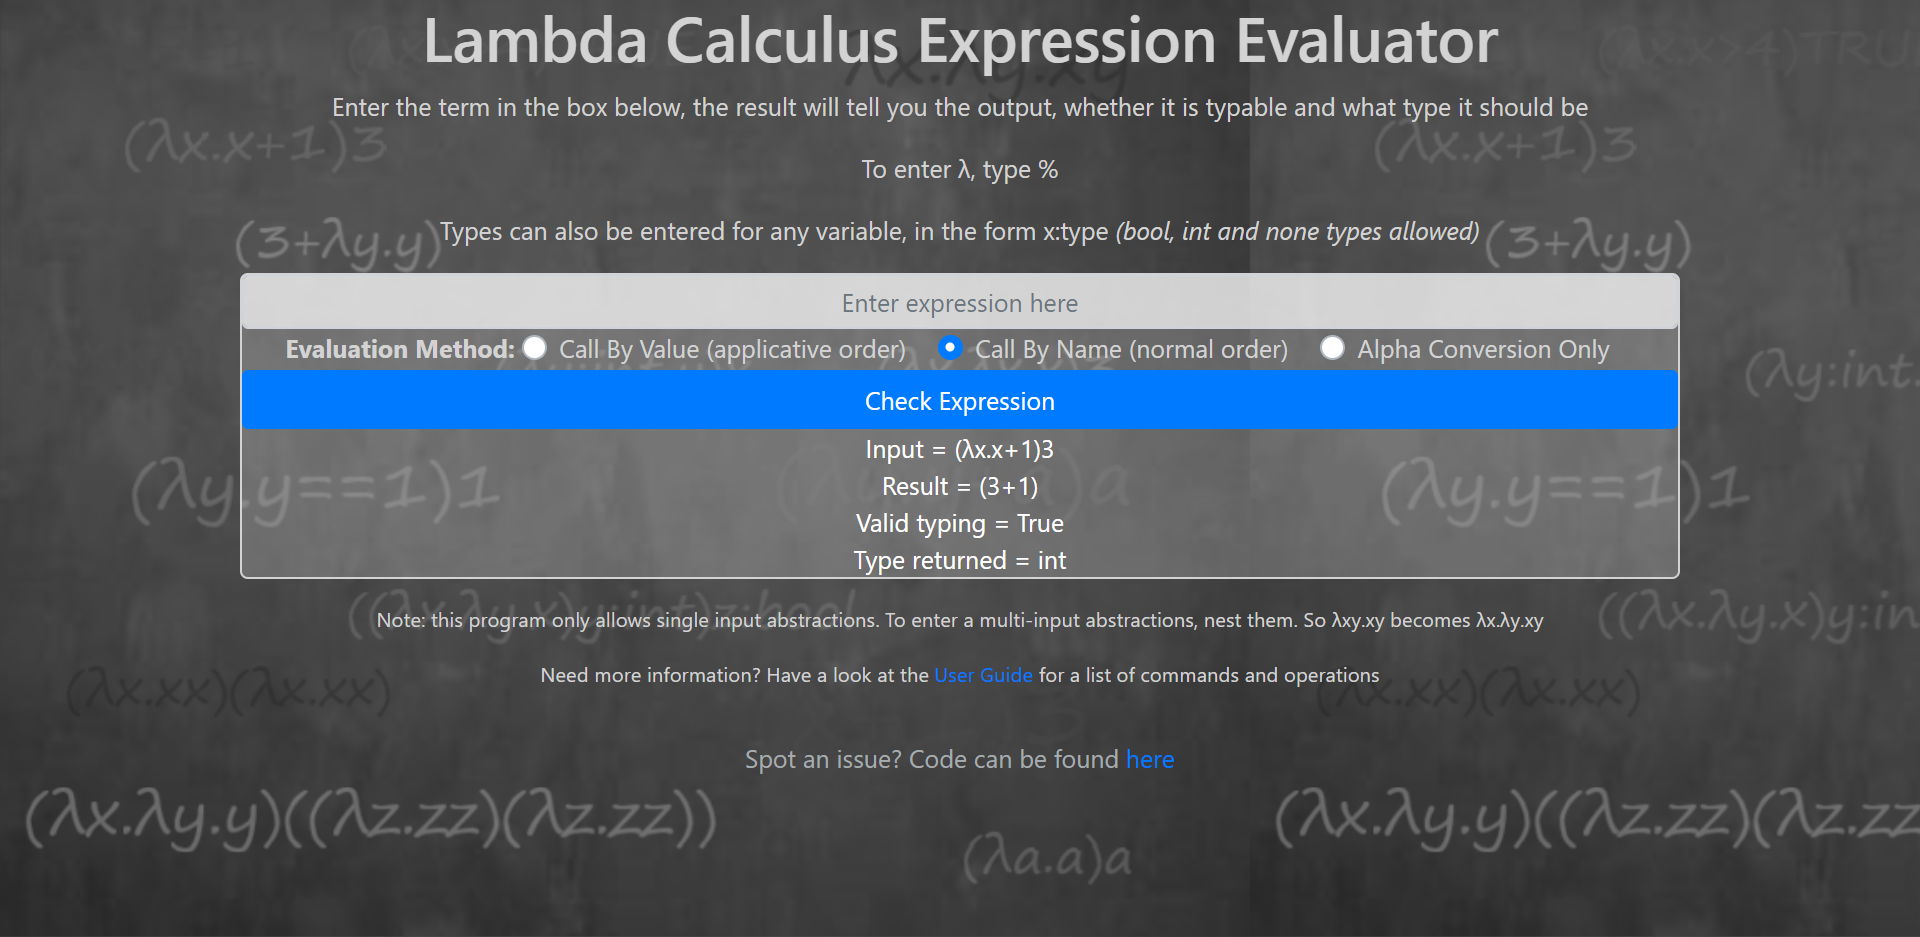
\includegraphics[scale=0.4]{images/web_interface_input}
	\caption{Web Interface With Returned Result}
	\label{web_interface_input}
\end{figure}

\begin{figure}[p]
	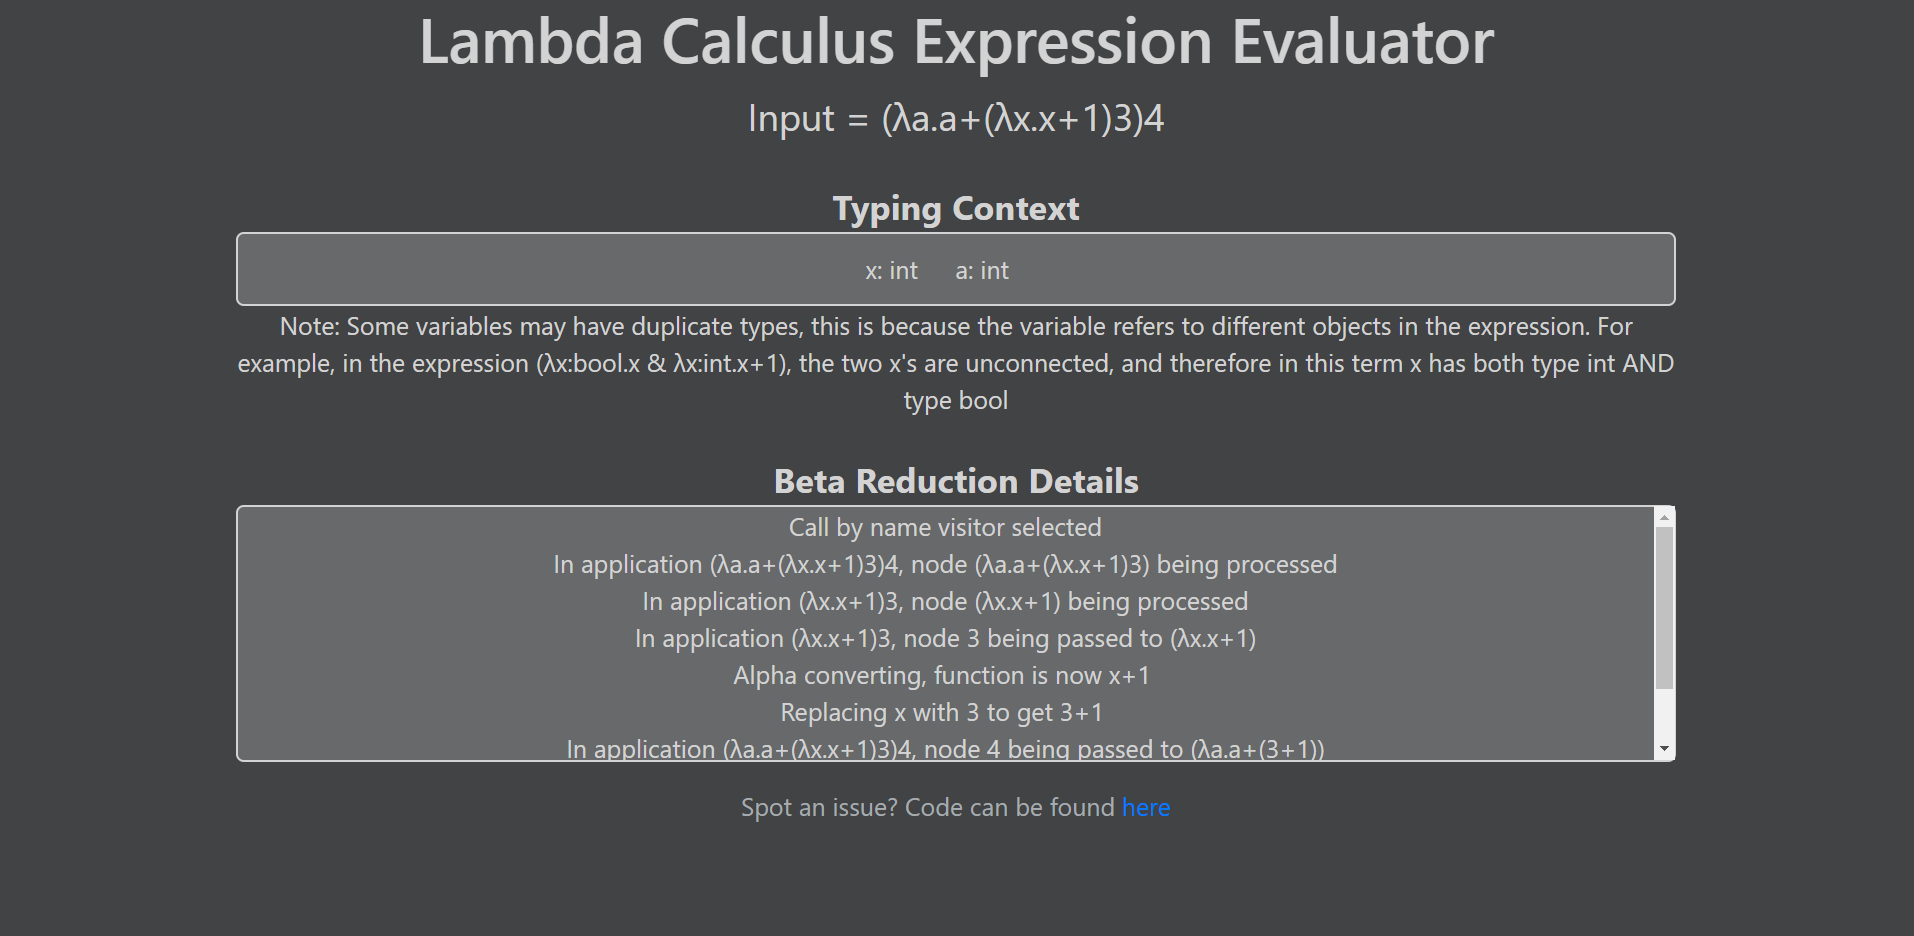
\includegraphics[scale=0.4]{images/web_interface_more_information}
	\centering
	\caption{Web Interface}
	\label{web_interface_more_information}
\end{figure}

\begin{figure}[p]
	\centering
	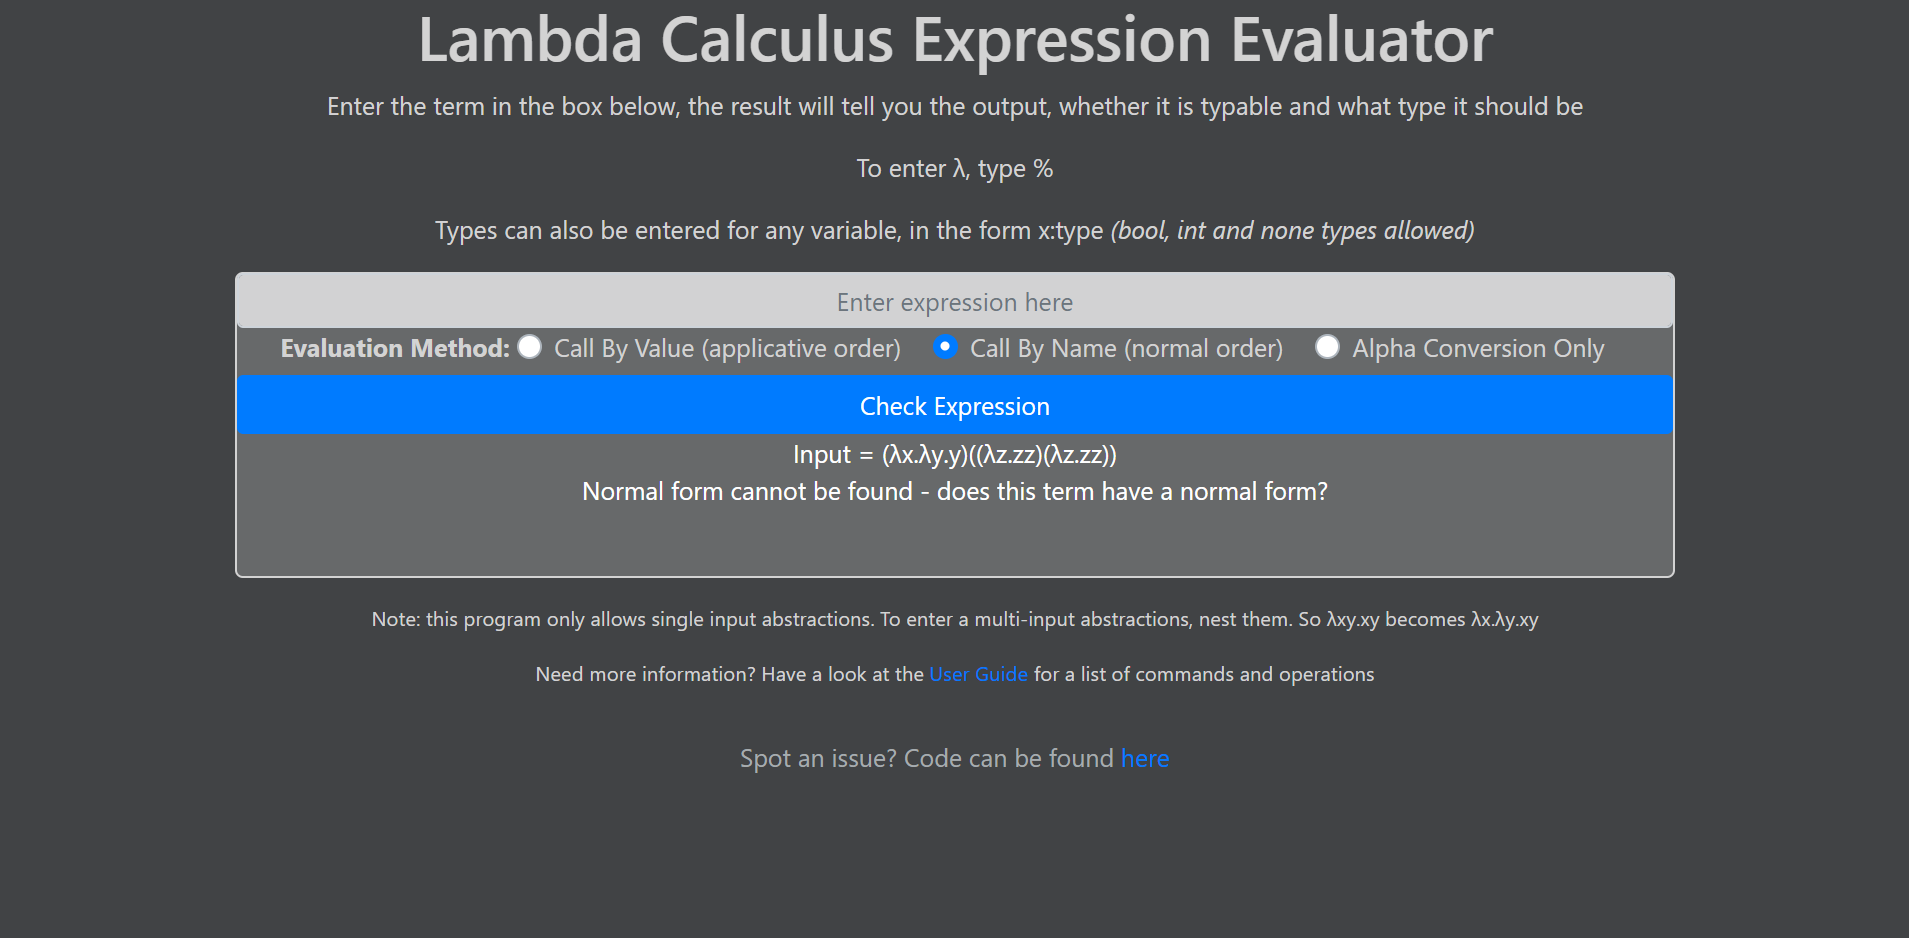
\includegraphics[scale=0.4]{images/web_interface_error}
	\caption{Web Interface With Error}
	\label{web_interface_error}
\end{figure}

\end{document}